\subsection*{Hướng phát triển trong thời gian tới}

Ngay từ giai đoạn đầu, các mô hình học máy như Logistic Regression, Random Forest, Support Vector Machine và Gradient Boosting đã được triển khai để phân loại tư thế ngủ với độ chính xác cao (lên đến 99.6\% với GB, 98.7\% với LR). Đồng thời, tác giả cũng đã thử nghiệm mô hình mạng nơ-ron nông (NN) và triển khai thành công trên vi điều khiển Arduino Nano 33 BLE Sense, mở đường cho khả năng chạy mô hình trực tiếp trên thiết bị nhúng.

Vì vậy, trong giai đoạn tiếp theo, tác giả sẽ tiếp tục áp dụng các mô hình học máy để cải thiện độ chính xác của hệ thống. Cụ thể, mô hình Logistic Regression (LR) — với ưu điểm về kích thước nhỏ và khả năng triển khai trên vi điều khiển — sẽ được tích hợp lên mạch phần cứng do nhóm tự thiết kế thay vì chỉ sử dụng bo mạch Arduino thương mại. Ngoài ra, việc sử dụng mô hình mạng nơ-ron đã được thực nghiệm trong khóa luận sẽ là cơ sở để mở rộng sang các mô hình học sâu (deep learning) nhẹ như CNN hoặc MobileNet nếu điều kiện phần cứng cho phép.

Bên cạnh đó, nhóm nghiên cứu đang xây dựng mạch nguyên lý và thiết kế mạch in trên phần mềm Altium, với mục tiêu hiện thực hóa một thiết bị tích hợp đầy đủ các thành phần: cảm biến, vi điều khiển, module truyền không dây và bộ xử lý tín hiệu.

\begin{figure}[htbp]
    \centering
    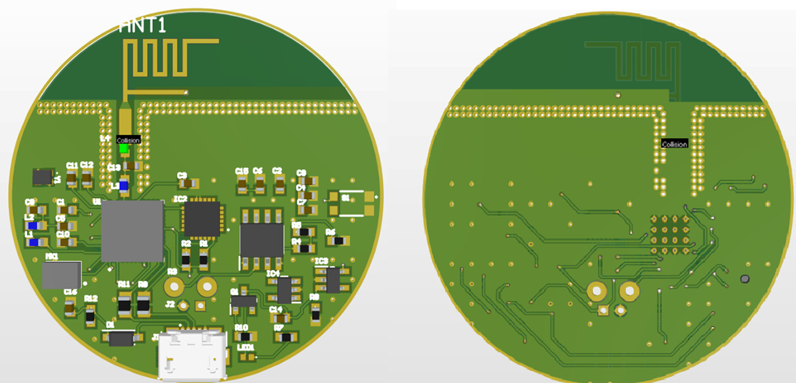
\includegraphics[width=0.75\linewidth]{images/macjh.png}
    \caption{Thiết kế mạch nguyên lý trên phần mềm Altium}
    \label{macjh}
\end{figure}

Hệ thống trong tương lai cũng sẽ được tích hợp thêm các tín hiệu sinh lý khác ngoài gia tốc, như cảm biến âm thanh, nhịp thở, độ bão hòa oxy máu,... nhằm hướng tới mục tiêu đánh giá chỉ số AHI (Apnea–Hypopnea Index) – một trong những thông số quan trọng trong chẩn đoán hội chứng ngưng thở khi ngủ (OSA).

Về mặt phần mềm, ứng dụng di động hiện tại hoạt động tốt nhưng còn hạn chế khi phải mở liên tục trong suốt quá trình ghi nhận. Để cải thiện trải nghiệm người dùng, tác giả đề xuất tích hợp module Wi-Fi vào phần cứng để gửi dữ liệu trực tiếp lên server. Khi đó, thiết bị di động sẽ chỉ cần hiển thị dữ liệu qua các ứng dụng chạy nền (foreground service) mà không cần mở ứng dụng chính thường xuyên, từ đó tiết kiệm năng lượng và tiện lợi hơn cho người dùng.

Về phía xây dựng tập dữ liệu, nhóm nghiên cứu đang khảo sát các phương pháp gán nhãn hiệu quả như:
\begin{itemize}
    \item Ghi hình bằng camera kết hợp đồng bộ thời gian;
    \item Gán nhãn hành động theo khoảng thời gian cố định;
    \item Gán nhãn trực tiếp trên ứng dụng di động thông qua nút bấm tích hợp.
\end{itemize}

Tác giả dự kiến phát triển một tính năng hỗ trợ gán nhãn trong ứng dụng di động nhằm hỗ trợ việc xây dựng tập huấn luyện có độ tin cậy cao phục vụ huấn luyện mô hình học máy.

\subsection*{Kết luận định hướng}

Mục tiêu dài hạn của nghiên cứu không chỉ dừng lại ở việc nhận diện tư thế ngủ, mà hướng đến phát triển một hệ thống HST (Home Sleep Testing) hoàn chỉnh phục vụ cho việc \textbf{đánh giá nguy cơ mắc hội chứng ngưng thở khi ngủ tắc nghẽn (Obstructive Sleep Apnea – OSA)}.

Tư thế ngủ là một trong những yếu tố quan trọng góp phần gây ra hoặc làm trầm trọng thêm tình trạng OSA, đặc biệt là ở các trường hợp OSA theo tư thế (positional OSA – pOSA). Do đó, việc nhận diện chính xác tư thế là bước nền cần thiết để xây dựng các mô hình tiên lượng hoặc gợi ý can thiệp lâm sàng.

Trong giai đoạn tiếp theo, hệ thống sẽ tiếp tục được mở rộng với mục tiêu:
\begin{itemize}
    \item Tích hợp thêm các loại cảm biến sinh lý như âm thanh (phát hiện ngáy), nhịp thở, nhịp tim, SpO\textsubscript{2}... để đánh giá gián tiếp các chỉ số liên quan đến ngưng thở;
    \item Phát triển thuật toán ước lượng chỉ số AHI (Apnea–Hypopnea Index) dựa trên tổng hợp tín hiệu;
    \item Thiết kế giao diện người dùng cho bác sĩ theo dõi từ xa và đề xuất hướng điều trị;
    \item Tối ưu mô hình học máy (như Logistic Regression hoặc mạng nơ-ron lượng tử hóa) để chạy trực tiếp trên vi điều khiển hoặc thiết bị đeo tay.
\end{itemize}

Tác giả kỳ vọng rằng trong tương lai gần, sản phẩm nghiên cứu có thể đóng vai trò như một thiết bị HST đơn giản, giá thành thấp, hỗ trợ các cơ sở y tế và người bệnh trong việc sàng lọc sớm và quản lý OSA một cách chủ động tại nhà – đặc biệt tại các khu vực thiếu điều kiện tiếp cận các thiết bị PSG tiêu chuẩn.
